
%%% Local Variables: 
%%% mode: latex
%%% TeX-master: t
%%% End: 

\chapter{凸包围体生成算法}
\label{cha:kcbp-construction}
从第~\ref{sec:convex-bv}~节可以看出包围体的紧致程度直接影响相应算法的效率,对于不规则形体, 常见的包围体往往不够紧致,凸包紧致但往往包含过多的面片数而增加算法的复杂性。

本文提出一种构造凸包围多面体的方法,该方法首先利用近似内凸包和~$k$-means~聚类算法生成构成凸包围多面体~$k$~个截面的法向。
然后根据输入点集沿各法向搜索切点构成截面, 最后由这些截面通过对偶映射的方式求交构成凸包围多面体。搜索截面过程中,各个法向的搜索过程相互独立互不影响,因此可以方便地利用~GPU~进行加速。
本文提出的方法的主要优势是:
\begin{inparaenum}[(1)]
\item 对给定点集可构造紧致的包围体;
\item 利用~GPU~加速,能够快速构造包围体;
\item 通过参数~$k$~调节凸包围多面体的简单性和紧致性,可适用于不同的应用场景。
\end{inparaenum}

由~$k$~个截面构成的凸包围多面体称为凸包围~$k$~面体($k$-Convex Bounding Polyhedron,简称~$k$-CBP), 可通过~$k$~个半空间定义:
\begin{equation}
\label{equ:kcbp_definition}
\left\{
\begin{array}{l}
    k\mbox{-CBP} = \mathop  \bigcap \limits_{i = 1}^k \bm{H_i} \\
    \bm{H_i} = \left\{ {\left. {\bm{p} \in {\mathbb{R}^3}} \right| \bm{n_i} \cdot \bm{p} \le {w_i}} , w_i \in \mathbb{R} \right\},
\end{array}
\right.
\end{equation}
其中,$\bm{n_i}$~是半空间~$\bm{H_i}$~的法向,方向指向包围体外部,
$w_i$~是输入点集中沿~$\bm{n_i}$~方向投影的最大值。
如图~\ref{fig:bunny}~所示是~Bunny~模型的凸包围~34~面体(34-CBP)。

\begin{figure}[htbp] 
\centering
  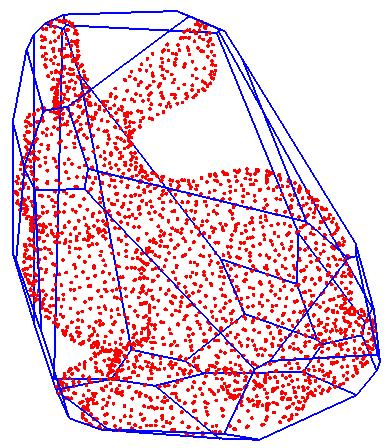
\includegraphics[width=1.5in]{bunny-34.png}
  \caption{~Bunny~模型的~34-CBP }
  \label{fig:bunny}
\end{figure}

本文算法的主要流程如图~\ref{lbl:kcbp-algorithm-flowchart}~所示,首先利用近似内凸包和~$k$-means~聚类算法生成构成凸包围多面体~$k$~个截面的法向,然后根据输入点集在~GPU~中沿各法向搜索切点构成截面,
最后由这些截面通过对偶映射的方式求交构成凸包围多面体。搜索截面需要多次扫描输入点集,在~CPU~中计算较耗时,因此用~GPU~加速使得算法整体性能得以提升,其他步骤在~CPU~计算即可。

\begin{figure}[htbp]
    \centering
    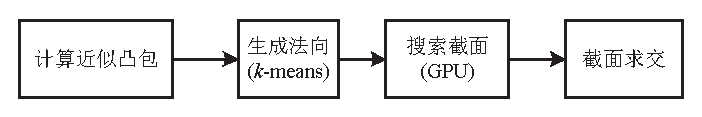
\includegraphics[width=5.5in]{kcbp-flowchart-x-aix.eps}
    \caption{构造~$k$-CBP~算法流程图}
    \label{lbl:kcbp-algorithm-flowchart}
\end{figure}

图~\ref{lbl:bunny-26-cbp-ch-ach}~从左至右分别显示了~Bunny~模型的~26-CBP、精确凸包和近似内凸包。
近似凸包是精确凸包的一种近似,与精确凸包外观相似但其构造复杂度降低,不少研究者利用该性质解决计算机图形学中很多问题\cite{hossain2013constructing}。

\begin{figure}[htbp] % use [htbp] to fix the position
\centering
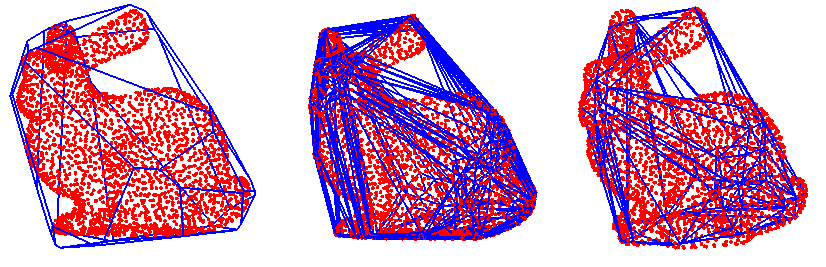
\includegraphics[width=5.0in]{26-bunny-ach-ch-kcbp.png}
\caption{~Bunny~模型的~26-CBP、凸包和近似内凸包}
\label{lbl:bunny-26-cbp-ch-ach}
\end{figure}

本文就利用了近似内凸包与精确凸包的相似性,从众多近似凸包面片的法向中通过~$k$-means~聚类算法生成构成凸包围多面体的~$k$~个法向。
本章后续部分将按步骤详细介绍算法的实现。
%由图可知, 近似内凸包的三角面片大致反映了精确凸包三角面片的分布情况,近似内凸包相应位置面积较大的三角面片对应到精确凸包的三角面片面积也较大, 因此该三角面片所在平面需尽量保留.

\section{截面法向的生成}
\label{sec:gen-normals}

截面法向的选定与多面体的紧致程度密切相关。
$k$-DOP\cite{klosowski1998efficient}~预先定义~$k/2$~对法向,且~$k$~值局限于6、14、18或26等少数几个,对于不同的模型其方向始终一致,导致其生成的多面体不能自适应模型,对于不规则形体的模型不够紧致。
与~$k$-DOP~相比,本文算法~$k$~值取值更灵活,因此可以根据不同需求不同应用场景更加灵活地选择需要的凸包围体。
根据经验,为了使凸包围多面体尽可能逼近凸包,在多面体数量一定的情况下需尽量保留凸包中面积较大的面。 
本文生成凸包围多面体的法向的流程是先通过一种线性算法\cite{bentley1982approximation}构造近似内凸包,然后从近似内凸包里选取面积最大的~$a$~个面的法向,最后用聚类算法从剩下的面中生成~$k-a$~个法向。
下面将介绍截面法向生成的主要步骤。

\subsection{近似内凸包生成聚类样本法向集}
\label{subsec:ach-gen-normals}

以平面点集的近似内凸包为例说明初始法向集的生成。

\begin{figure}[htbp]
  \centering
  \subcaptionbox{分组\label{lbl:subfig-split-groups}}{
    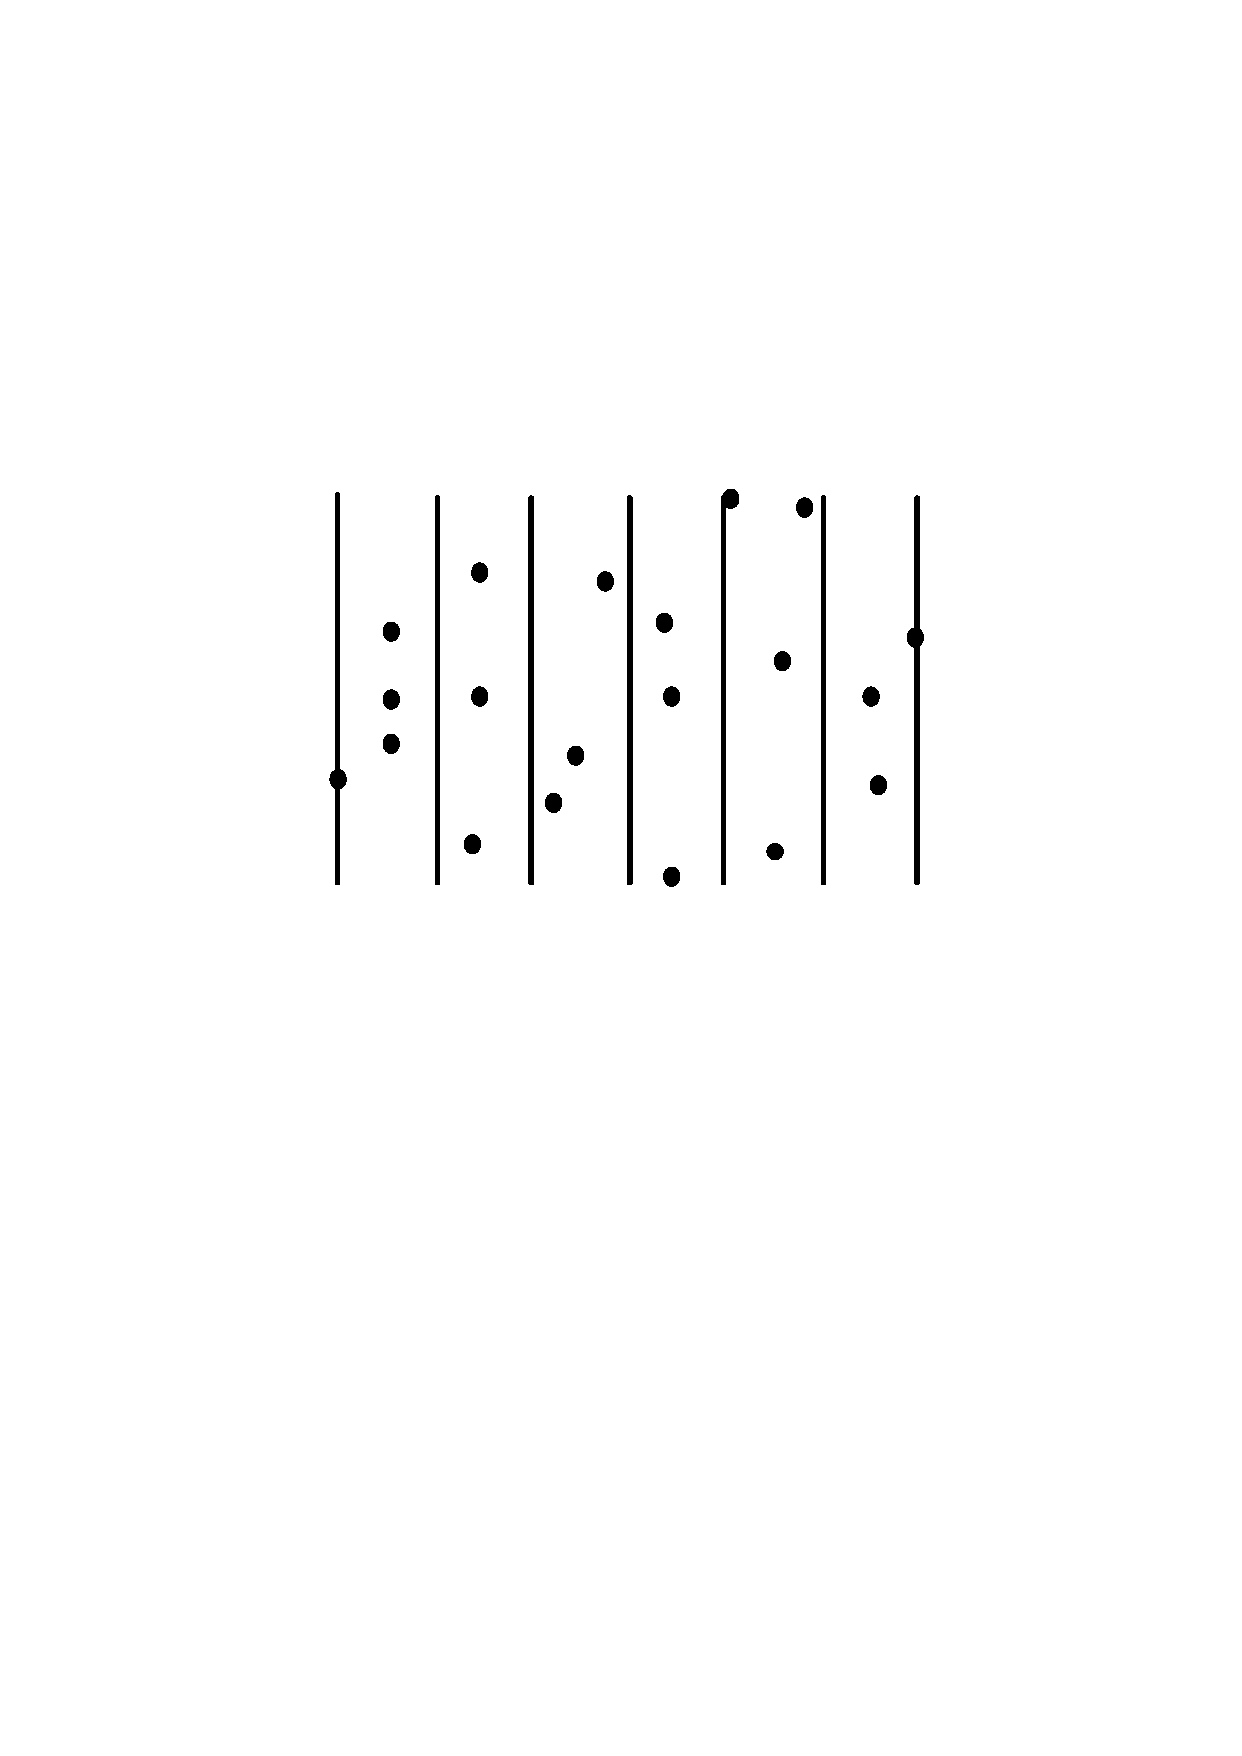
\includegraphics[width=2.2in]{approximate-convexhull-step1.pdf}} \hspace{0.5cm}
  \linebreak
  \subcaptionbox{选极值点\label{lbl:subfig-find-extrems}}{%
    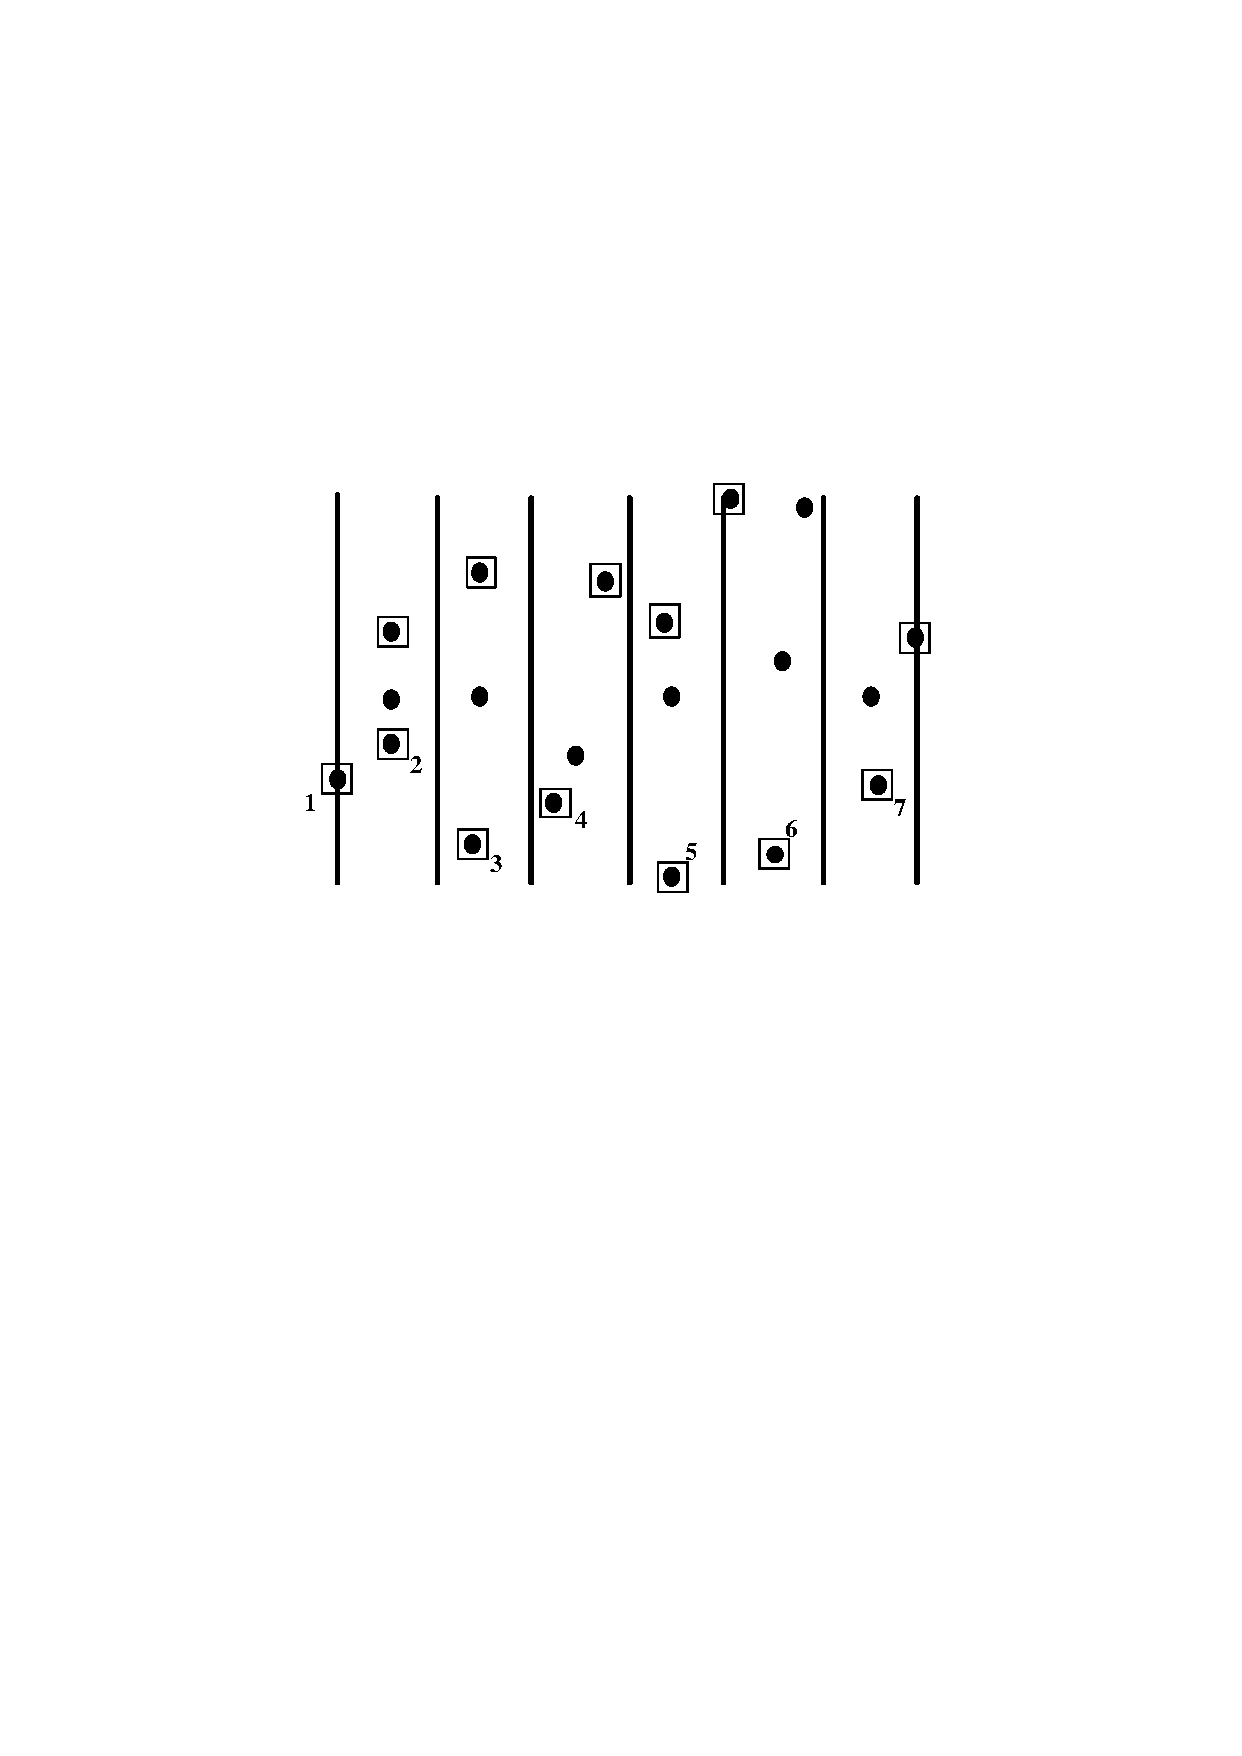
\includegraphics[width=2.2in]{approximate-convexhull-step2.pdf}} \hspace{0.5cm}
  \hspace{2em}
  \subcaptionbox{连线\label{lbl:subfig-connect-extremes}}{%
    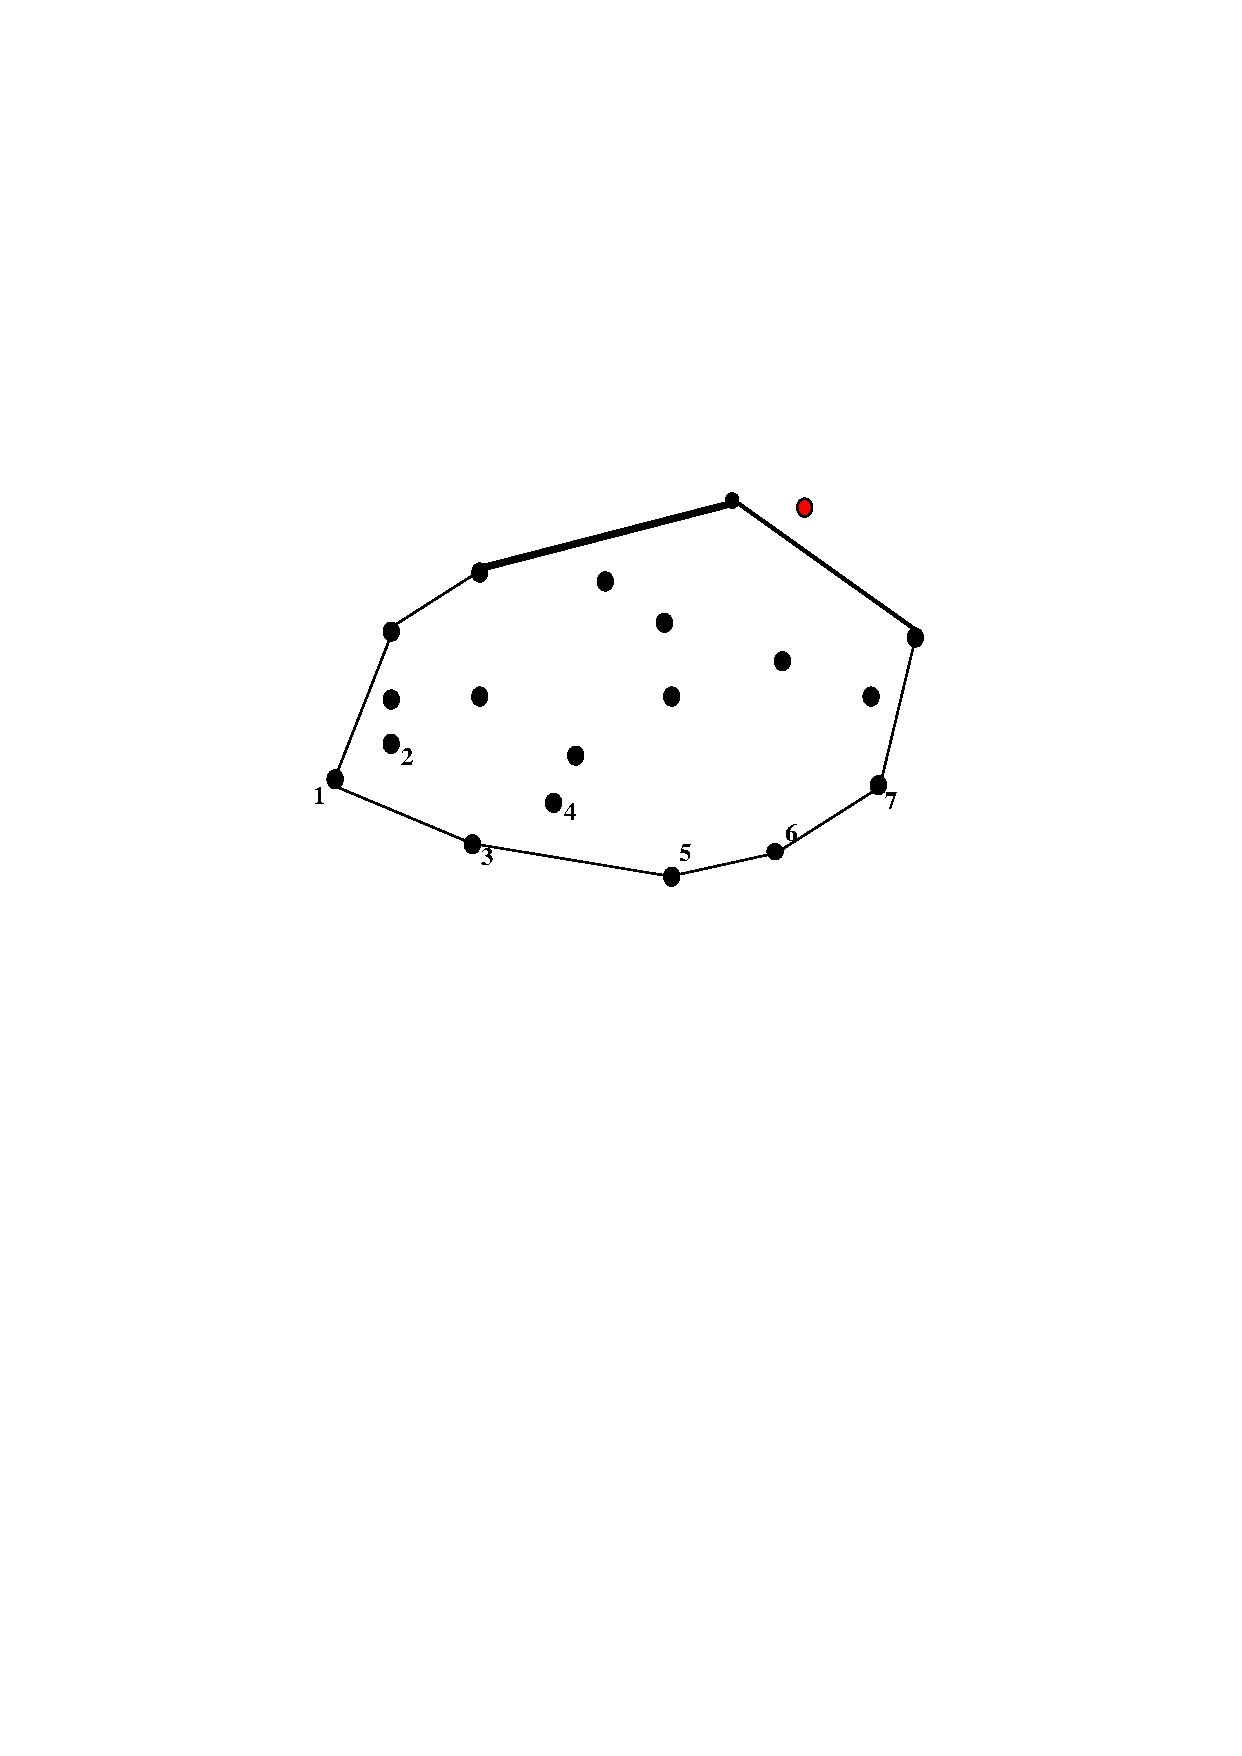
\includegraphics[width=2.2in]{approximate-convexhull-step3.pdf}} \hspace{0.5cm}
  \caption{二维近似内凸包的构造\cite{bentley1982approximation}}
\label{lbl:ach-2d}
\end{figure}

如图~\ref{lbl:ach-2d}~所示,整个算法分为如下3个步骤:

\begin{inparaenum}[(1)]
%\begin{enumerate}[(1)]
\item \textbf{分组:}
首先根据~$x$~轴将输入点集均分~$\xi$~组,如图~\ref{lbl:subfig-split-groups}所示,$\xi$值可以根据输入点集数量以及希望得到的近似凸包的近似程度进行选取,图示中分成了~6~组。\\
\indent \item \textbf{选极值点:}
然后在每组中找出沿~$y$~轴的最大最小坐标值的点,得到每组的极值点,如图~\ref{lbl:subfig-find-extrems}~所示,在边界上的点可直接当作极值点。\\
\indent \item \textbf{连线:}
最后按条件连接每组的最值构成近似内凸包,如图~\ref{lbl:subfig-find-extrems}所示,以下半圈为例,在选定的极值点中先选定最左边的点~1,下一个候选点~2,连接~13~发现候选点~2~在~13~的左边,丢弃候选点~2~直接连接~13,同理连接~35,
当查看候选点~6~时,发现点~6~在~57~连线的右边,因此候选点~6~保留,依次类推可得整个下半圈为凸包,上半圈同理可得。最后合并上下半圈得到如图~\ref{lbl:subfig-connect-extremes}所示的结果。
\end{inparaenum}
%\end{enumerate}

此算法复杂度为~$O(n+\xi)$。  
得到近似凸包后,因较长的边(图~\ref{lbl:subfig-connect-extremes}~中的粗边)对最后凸包围多边形影响较大, 因此可以保留较长的~$a$~条边, 其他~$n-a$($n$~为近似内凸包边数)进行聚类得到~$k-a$~类, 最后得到边对应的垂直向外的方向作为法向。
在三维空间里, 可按照~$x,y$~轴最多划分成~$(\xi+2)\times (\xi+2)$~个网格, 每个网格取~$z$~轴的最大最小坐标值, 因此所有网格含最多有~$2(\xi+2)^2$~个极值点, 其凸包可以在~$O(\xi^2\log \xi^2) = O(\xi^2\log \xi)$~内求得, 因此整个算法时间复杂度为~$O(n+\xi^2\log\xi)$, 
关于此算法更详细的细节可参考文献~\onlinecite{bentley1982approximation}。 实验过程中, 为了更快地构造近似内凸包, $\xi$~值通常取得较小(例如取~$\xi=10$)。

假设点~$A,B,C$~为近似凸包的某个平面~$P_i$~上逆时针方向上的3个顶点,则该平面~$P_i$~的法向~$\bm{n_i}
= \overrightarrow{AB} \times
\overrightarrow{AC}$,这些法向就是参与聚类算法的所有样本法向集。

\subsection{聚类初始点的选择}
\label{subsec:initial-normals}

聚类算法是数据挖掘领域里的研究热点之一,$k$-means~是最流行和最简单的基于划分的聚类算法\cite{Jain2010}。其中,$k$-means
算法最初的步骤就是初始聚类中心的选择。本文算法将采取如下的策略生成:给定一个单位球,将其按照等面积划分成$k$份即$k$-means中的参数$k$,连接球心到每份中心点构成的方向作为法向,其效果如图~\ref{lbl:kmeans-init-normals-26}~所示($k=26$)。

\begin{figure}[htbp]
    \centering
    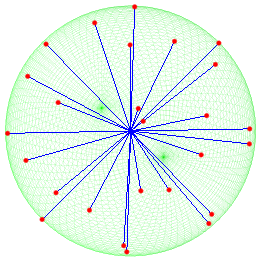
\includegraphics[height=1.7in]{kmeans-init-normals-26.png}
    \caption{初始聚类法向的生成}
    \label{lbl:kmeans-init-normals-26}
\end{figure}
初始点生成算法具体如算法~\ref{alg:get_init_normals_by_area}~所示\footnote{http://www.cmu.edu/biolphys/deserno/pdf/sphere\_equi.pdf}。
另外,亦可使用如文献~\onlinecite{wong1997sampling}~中的数学统计方法在球面上生成若干个点使其满足均匀分布。

\begin{algorithm}[htbp]
\small
\caption{初始法向的生成}
\label{alg:get_init_normals_by_area}
\begin{algorithmic}[1]
\Require
初始法向数量$k$
\Ensure
~$k$~个法向 $normals$

\Function{GenerateInitNormal}{$k$}
  \State $area \leftarrow 4\pi / k$
  \State $m\_v \gets \Call{round}{\pi/\sqrt{area}}$
  \State $d\_v \gets \pi/m\_v$
  \State $d\_phi \gets area/d\_v$
  \For {$m=0 \to m\_v-1$}
      \State $v \gets \pi m/m\_v$
      \State $m\_phi \gets \Call{round}{2\pi\sin{v}/d\_phi}$
      \For {$n=0 \to m\_phi-1$}
          \State $\phi \gets 2\pi n/m\_phi$
          \State $normals \gets normals \cup \Call{vec3}{\sin{v}\cos{\phi},\sin{v}\sin{\phi},\cos{v}}$
      \EndFor
  \EndFor
  \State \Return $normals$
  \EndFunction
\end{algorithmic}
\end{algorithm}
 
\subsection{聚类确定法向}
\label{subsec:determ-normals}

聚类算法将相似程度高的变量聚集到一类,距离度量是$k$-means中的关键,采用不同的距离计算函数可能得到不同的聚类结果,依据数据的不同性质可选用不同的距离度量方法,常用的有欧式距离,曼哈顿距离和卡方距离等等。
本文采用余弦距离度量,将方向相近的点归聚到一类。$k$-means~本质上是一个迭代贪心算法,每一次迭代需要重新计算每一类的中心点,直到两次迭代后中心点相差在给定的容差范围内为止。
完整的算法如算法~\ref{alg:kmeans-determine-normals}~所示。

\begin{algorithm}
\small
\caption{$k$-means~确定法向}
\label{alg:kmeans-determine-normals}
\begin{algorithmic}[1]
\Require
初始中心点 $init$, 聚类数量 $k$, 聚类样本法向集 $points$
\Ensure
~$k$~个聚类后的法向 $result$
\Function{kmeansCluster}{$init, k, points$}
  \ForAll {$p \in points$}
    %\State $tmp \gets -\infty $
    \ForAll {$c \in init$}
        \State $\phi \gets c \cdot p$ \Comment{计算余弦距离, 并记录每个聚类变量属于哪一类}
        %\State $tmp \gets max(tmp, \phi)$ \Comment{记录每个聚类变量属于哪一类}
    \EndFor
    \ForAll {$c \in init$}
    \State $result \gets \Call{update}{c}$ 
        \Comment{按照公式(\ref{equ:kmeans-update-center})更新中心点}
        \If{$ \Call{checkState}{result, init, iter}$}
        \State \Return {$result$}
        \State \Comment{检测迭代条件是否满足,中心点容差范围内不在变化或迭代次数超过最大迭代次数}
    \Else
        \State $init \gets result $
        \State $iter \gets iter+1 $
    \EndIf
    \EndFor
  \EndFor
\EndFunction
\end{algorithmic}
\end{algorithm}

算法~\ref{alg:kmeans-determine-normals}~中第7行~$UPDATE$~方法作用是聚类迭代更新每类的中心点,
本文更新中心点时将每个法向对应的面片的面积作为权重即
\begin{equation}
\label{equ:kmeans-update-center}
\bm{c_i}=\frac{\sum_{i=1}^{i=n} \omega_i \cdot \bm{n_i} } {\sum_{i=1}^{i=n} \omega_i}
,
\end{equation}
其中,$\bm{c_i}$~为第~$i$~类的中心点,$\omega_i$~为法向~$\bm{n_i}$~所在面片对应的面积,这样使得生成的法向尽量靠近原始近似凸包面积较大的面片的方向。

通过用聚类方法得到的法向生成的凸包围多面体比直接用初始法向生成的包围体更加紧致。
如图~\ref{lbl:kemans-fixed-kcbp}~所示, 
其中图~\ref{lbl:fixed-kcbp-bunny}~为按照初始方向为~Bunny~模型生成的凸包围多面体,其中~$k=26$。
聚类后其法向及其生成的凸包围多面体如图~\ref{lbl:kmeans-kcbp-bunny}~所示,后者的紧致程度比前者高~14.98\%。

\begin{figure}[htbp]
\setcounter{subfigure}{0}
  \centering
  \subcaptionbox{初始法向生成$k$-CBP\label{lbl:fixed-kcbp-bunny}}{%
    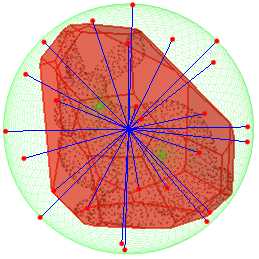
\includegraphics[width=1.8in]{kmeans-init-normals-26-for-bunny.png}}\hspace{3em}%
  \subcaptionbox{聚类法向生成$k$-CBP\label{lbl:kmeans-kcbp-bunny}}{%
    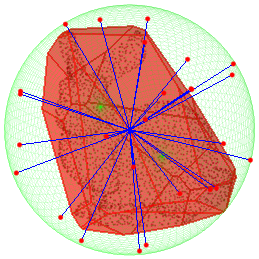
\includegraphics[width=1.8in]{kmeans-cluster-normals-26-for-bunny.png}}\hspace{3em}%
  \caption{初始法向和聚类确定法向生成$k$-CBP对比($k=26$)}
  \label{lbl:kemans-fixed-kcbp}
\end{figure}

\section{搜索截面}
\label{sec:search:planes}

在确定构成~$k$-CBP~的法向后,只需要搜索空间上的一个点即可确定
~$k$-CBP~的截面,搜索截面等效于寻找沿着法向上的最大投影值,即对每个法向~$\bm{n_i}$,从输入模型的所有点中寻找最大投影值的点作为切点进而确定法向~$\bm{n_i}$~对应的截面。
具体算法如算法~\ref{alg:search-plans-cpu}~所示,该过程的时间复杂度为~$O(k\cdot
n)$, 其中~$k$~为法向数量,$n$~为模型点的数量。

\begin{algorithm}[htbp]
\small
\caption{搜索截面串行算法}
\label{alg:search-plans-cpu}
\begin{algorithmic}[1]
\Require
截面法向 $normals$, 模型点集 $points$
\Ensure
多面体截面 $planes$
\Function{SearchCuttingPlanes}{$normals, points$}
  \ForAll {$\bm{n} \in normals$}
      \ForAll {$\bm{p} \in points$}
          \State $proj \gets  \bm{p} \cdot \bm{n}$ \Comment{计算投影值}
          \State $max\_proj \gets \Call{max}{proj, max\_proj}$ \Comment{更新最大投影值}
      \EndFor
  \EndFor
  \ForAll {$\bm{n} \in normals$}
      \State $max\_point \gets \bm{n} \cdot max\_proj$ \Comment{切点}
      \State $planes\gets planes \cup \Call{plane}{\bm{n}, max\_point}$ \Comment{构造平面}
  \EndFor
  \State \Return $planes$
\EndFunction
\end{algorithmic}
\end{algorithm}

从算法~\ref{alg:search-plans-cpu}~可以看出该搜索过程中各法向的计算相互独立,互不影响,因此可方便地借助~GPU~并行加速。
本文将采用两种平台进行~GPU~加速,一种平台是基于~OpenGL~着色语言,另外一种是~CUDA~平台,下面将分别介绍这两种平台的实现。

\subsection{基于着色器的并行算法}
\label{subsec:determ-normals-by-shader}

OpenGL~提供了可编程管线,它的轻便性、跨平台性和被广泛硬件厂家所支持使得~OpenGL~着色语言(OpenGL Shading Language,简称~GLSL)被广泛应用,在基于~GPU~的通用计算(General
Purpose Graphic Process Unit,简称~GPGPU)中也发挥着重要作用。下面将分别介绍本文提出的基于深度缓冲(Z Buffer)和乒乓技术的算法。

\subsubsection{基于深度缓冲的算法}
	
在~OpenGL~中,当渲染~3D~模型时,深度测试是在片段着色器工作后的一个重要测试操作,当两个片段在相同的位置时,深度测试的目的是决定哪个片段将要保留下来,默认情况下,最前面即有较小(或较大,可设置)的~$z$~坐标值的片段将通过测试被保留下来。
每个片段的深度信息保存在深度缓冲中,当新的片段通过测试后将更新缓冲中的值。
本文充分利用了~OpenGL~的这种机制,算法每走一遍渲染流程将找出一个方向上的切点,在顶点着色器中,将所有点的~$x,y$~坐标值设为一样,并将该点在法向上的投影作为~$z$~值即深度值,所有点经过深度测试后将只有~$z$~值最大的点被保留下来,该点就是沿着这个法向的切点。该过程的算法流程图如~\ref{fig:flowchart:zbuffer}~所示。

\begin{figure}[htbp]
  \centering
  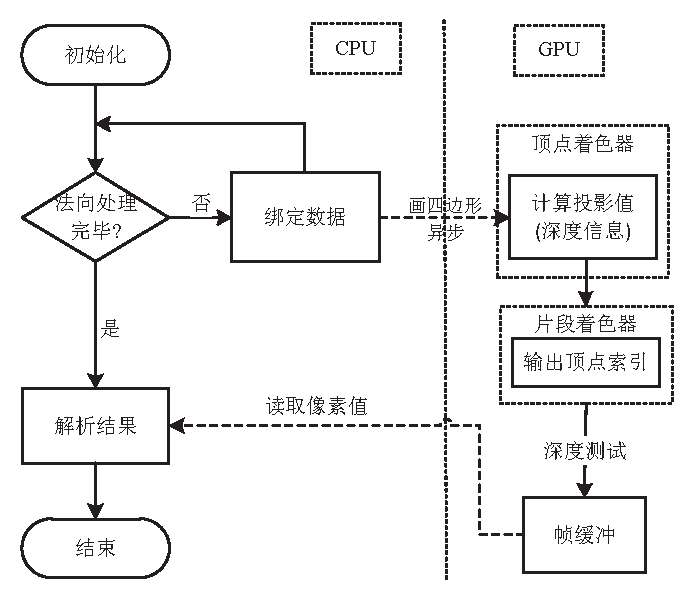
\includegraphics[width=4.0in]{shader-z_buffer.eps}
  \caption{基于~Z Buffer~算法流程图}
  \label{fig:flowchart:zbuffer}
\end{figure}

在实际实现过程中需要注意默认情况下~OpenGL~处理~$x$~和~$y$~坐标值的范围是~$[-1,1]$,而深度值需要映射到~$[0,1]$。我们利用一张~$k \times 1$~大小的纹理保存结果,将第~$i$~个法向的切点保存在纹理的~$(i,0)$~坐标处,
这样做的好处是每绘制一遍不用清除深度缓冲,最后可以一次性读取这个~$k \times 1$~大小的纹理得到结果。
如代码~\ref{shader:zbuffer}~的着色器代码所示,OpenGL~中利用齐次坐标处理渲染流程,因此我们利用前三个分量保存法向的~$x,y,z$~坐标值,第4个分量~$w$~保存法向的索引,在片段着色器中,只需要简单地输出切点的在输入点数组的索引即可。
通过绘制~$k$~遍,我们从大小为~$k \times 1$~的纹理中读出点索引以此就能确定~$k$~切平面,每绘制一遍得到1个切平面,当~$k$~值较大时,这个过程仍然比较耗时,从实验结果也能看出,这种算法适用于~$k$~值相对较小的情况。

%\lstinputlisting[language={shader}, caption={Vertex shader(Z buffer algorithm)}, label=vertex_shader_zbuffer]{shader_zbuffer.vert}
\lstinputlisting[language={shader}, caption={基于~Z Buffer~算法着色器代码}, label=shader:zbuffer]{shader_zbuffer.vert}

\subsubsection{基于乒乓技术的算法}

渲染到纹理(Render To Texture,简称~RTT)是一个非常重要的图形可视化技术,它能够帮助快速地渲染很多漂亮的结果,同时也是~GPGPU~重要组成部分。在基于~OpenGL~的~GPGPU~中,通常要将参与计算的数据通过~CPU~传送至~GPU~的特定大小的纹理中,
通过绘制一个与保存数据有着同样大小的四边形来调用着色器中的算法\cite{gpgpuqiu},将结果输出到纹理中。该过程中,绘制同样大小的四边形是为了避免纹理插值对输入数据的影响。
RTT~的算法一般是在片段着色器(Fragment Shader)中完成,有时通过一遍的绘制得不到最终结果还需要把前一次运算结果传递给下一次运算用来作为后继运算的输入,此时可以利用乒乓技术来解决。

\begin{figure}[htbp]
  \centering
  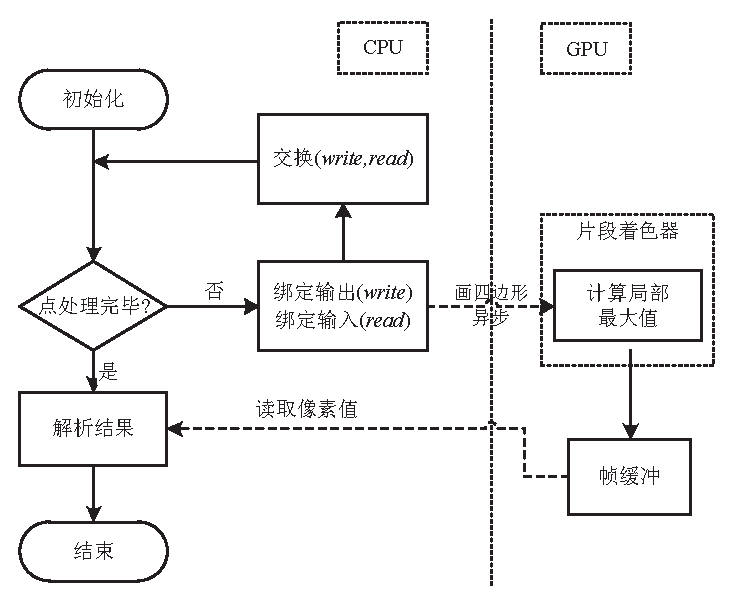
\includegraphics[width=4.2in]{shader-rtt_pp.eps}
  \caption{基于乒乓技术算法流程图}
  \label{fig:shader-rtt-pingpong-flowchart}
\end{figure}

图~\ref{fig:shader-rtt-pingpong-flowchart}~为基于乒乓技术的算法的流程图,算法将所有法向保存在纹理~$read$~中并利用纹理~$write$~缓存中间结果,第~$m$~次渲染进行计算时,纹理~$read$~作为输入,将渲染即计算的结果缓存在纹理~$write$~中,
在第~$m+1$~次渲染时将读取缓存在纹理~$write$~中的数据作为输入,而此时纹理~$read$~又作为输出,如此进行交替,每步交换只更改沿着每个法向的局部最大值。
如代码~\ref{shader:pingpong}~中的片段着色器代码所示,用一个像素值保存法向的~$xyz$~坐标值和沿着该法向投影得到最大值,另外该像素的第四个分量保存该最大值点在输入点数组中的索引。
算法将输入点分成~$x$~份,每次只处理一份,在当前渲染过程中,找出在该批点集中沿着所有法向投影值最大的点,当处理下批点集即下一次渲染时,将与上次局部最大投影值进行比较,若有新的投影最大值就更新,如此反复~$x$~次,
当所有点都被处理完毕后得到沿着所有法向投影最大值的点即切点。最后再通过~CPU~一次性从帧缓冲中读取所有法向的切点。

\lstinputlisting[float=!ht, language={shader}, caption={基于乒乓技术算法着色器代码}, label=shader:pingpong]{shader_rrt_pingpong.frag}

与~Z Buffer~算法相比,基于乒乓技术的算法在进行一次绘制操作能够得到沿着~$k$~个法向的局部(所有处理过的点集)最大值。为了充分利用~GPU~的并行计算能力,将每次处理点的数量设置为~GPU~硬件所支持的~OpenGL~中统一块(uniform
block)所能容纳数据的大小,即需要反复绘制的次数为~$x=n/b$,其中~$n$~为点集大小,$b$~为统一块能容纳点的数量,值与显卡具体型号有关。 

\subsection{基于~CUDA~的并行算法}
\label{subsec:determ-normals-by-cuda}

~CUDA~是显卡公司~NVIDIA~推出的通用的并行计算架构平台,能够利用~GPU~解决并行计算问题,并提供了多种语言的编程接口。
CUDA~程序可以由一系列的主机程序组成,主机程序能够并行地在~GPU~设备上运行,GPU~运算单元将并行的线程分解成线程块,每个线程块又由若干线程组成,GPU~的流水处理器以线程块为单位进行调度。
将问题划分成子问题提交给~GPU~让多线程同时处理这些子问题,这样可以提升算法的效率\cite{lauterbach2009fast}。

如图~\ref{lbl:reduction-getmax}~所示,最大投影值的计算可采用如下规约方式:将输入点交给数量为~$t$~的线程计算点积得到投影值,
线程~$i$~和~$i+t/2$~比较选取较大者,经~$\log_2t$~次比较可得最大值。

\begin{figure}[htbp] % use [htbp] to fix the position
\centering
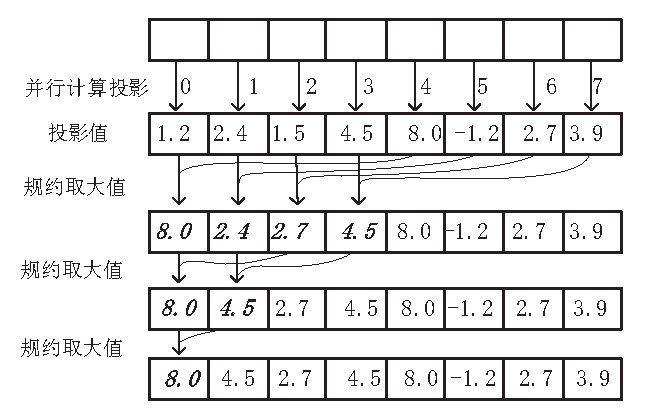
\includegraphics[width=4.2in]{gpureduction.eps}
\caption{并行规约求最大投影值}
\label{lbl:reduction-getmax}
\end{figure}

图~\ref{lbl:reduction-getmax}~所示的示例中,假设有~8~个点与某法向点积得到的投影值为~$(1.2,2.4,1.5,4.5,8.0,-1.2,2.7,3.9)$,有4个线程~同时比较第~$i$~个投影值与~$i+4$~投影值得到新的较大投影值~$(8.0,2.4,2.7,4.5)$,并将新的较大的投影值放入线程~$i$~中,
再以同样的方式规约得到较大的两个投影值~$(8.0,4.5)$,最后再通过一次比较得到最大的投影值~$8.0$~。
文献~\onlinecite{Harris2007Optimizing}介绍了更多更详细规约优化技术。

\section{截面求交算法}
\label{sec:intersect-planes}

确定~$k$-CBP~各个截面后,直接求得所有平面的交点并排除在平面外部的交点即可得到~$k$-CBP~的顶点。该问题即转化为:给定~$k$~个平面及其法向,平面及法向相当于一个半空间~$\bm{H}$,即已知集合$\{\bm{H_1},
\bm{H_2}, \cdots, \bm{H_k}\}$,求$\bm{H_1} \cap \bm{H_2} \cap \cdots
\cap \bm{H_k}$。该问题是一个线性规划(Linear Programming)问题,文献~\onlinecite{dengcg}~详细介绍了在二维线性规划下的相关算法,本文将分别采用一种直观的枚举算法和利用对偶映射的方法求得~$k$-CBP~的交点。

\subsection{枚举法}
\label{subsec:intersection-enum-geometry}

空间中的平面位置情况如图~\ref{fig:three-planes-intersection}~所示,可分为如下几种情况:
\begin{inparaenum}[(1)]
\item \textbf{无交点} 若3个平面互相平行则没有交点,如图~\ref{lbl:intersection-center-0}~;
\item \textbf{1~条交线} 如图~\ref{lbl:intersection-center-1}~所示,3个平面相交于~1~条交线;
\item \textbf{2~条交线} 当有两个平面互相平行,另一个平面与其相交时有2条交线,如图~\ref{lbl:intersection-center-2}~;
\item \textbf{3~条交线} 如图~\ref{lbl:intersection-center-3}~所示,3个平面交于~3~条交线;
\item \textbf{1~个交点} 最后一种情况是三个平面相交于1点的情况,如图~\ref{lbl:intersection-center-4}~所示。
\end{inparaenum}

一个凸多面体的每一个顶点都可看作是至少3个平面的交点。现在只需要枚举出所有3个平面相交于1点的所有情况即可得到$k$-CBP~的顶点,值得注意的是,并非所有交点都是多面体的顶点,交点在某个半空间的正方向上即在半空间相交区域的外部须排除。

\begin{figure}[htbp]
  \centering
  \subcaptionbox{没有交点\label{lbl:intersection-center-0}}{%
    
\includegraphics[width=1.8in]{intersection-center-0.png}}\hspace{1em}%
  \subcaptionbox{交于~1~条线\label{lbl:intersection-center-1}}{%
    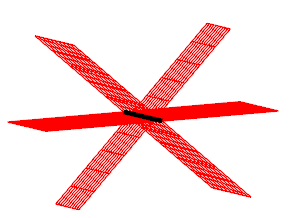
\includegraphics[width=1.8in]{intersection-center-1.png}}\hspace{1em}%
  \subcaptionbox{交于~2~条线\label{lbl:intersection-center-2}}{%
    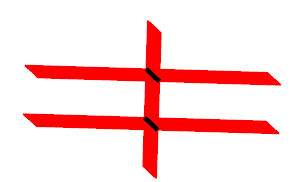
\includegraphics[width=1.8in]{intersection-center-2.png}}%
  \\
  \subcaptionbox{交于~3~条线\label{lbl:intersection-center-3}}{%
    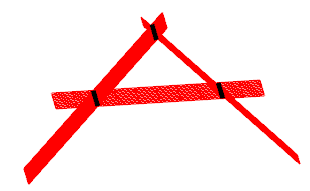
\includegraphics[width=2.3in]{intersection-center-3.png}}%
  \subcaptionbox{交于~1~个点\label{lbl:intersection-center-4}}{%
    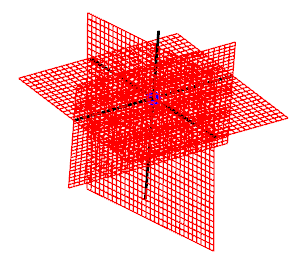
\includegraphics[width=2.0in]{intersection-center-4.png}}%
  \caption{空间中~3~个平面的相交情况}
  \label{fig:three-planes-intersection}
\end{figure}

假设满足如图~\ref{lbl:intersection-center-4}~所示的三个平面的法向分别是$\bm{n_1}, \bm{n_2}, \bm{n_3}$,
平面上一点分别为~$\bm{p_1}, \bm{p_2}, \bm{p_3}$,则三个平面的交点须满足如下方程: 
\begin{equation}
  \label{equa:three-planes-intersection}
  \left\{
    \begin{array}{l}
      \bm{n_1} \cdot \bm{x} = \bm{n_1} \cdot \bm{p_1}\\
      \bm{n_2} \cdot \bm{x} = \bm{n_2} \cdot \bm{p_2}\\
      \bm{n_3} \cdot \bm{x} = \bm{n_3} \cdot \bm{p_3}
    \end{array}
    \right.
\end{equation}

令$(\bm{n_1} \cdot \bm{p_1}, \bm{n_2} \cdot \bm{p_2}, \bm{n_3} \cdot \bm{p_3})
= (y_1, y_2, y_3) = \bm{y}$,则求解式(\ref{equa:three-planes-intersection})相当于解线性方程组
$\bm{A} \bm{x}=\bm{y}$ 即 $(\bm{n_1},\bm{n_2}, \bm{n_3})^T \cdot \bm{x} = \bm{y}$, 令
$\bm{n_i} = (a_{i1}, a_{i2}, a_{i3}), i=\{1,2,3\}$,则有:
\begin{equation*}
  \label{equa:matrix:crammer}
  \left(
    \begin{array}{ccc}
      a_{11} & a_{12} & a_{13} \\
      a_{21} & a_{22} & a_{23} \\
      a_{31} & a_{32} & a_{33} \\
    \end{array}
  \right)
  \cdot 
  \bm{x} 
 % \left(
 %   \begin{array}{c}
 %     x_{1} \\
 %     x_{2} \\
 %     x_{3} \\
 %   \end{array}
 % \right)
  =
  \left(
    \begin{array}{c}
      y_{1} \\
      y_{2} \\
      y_{3} \\
    \end{array}
  \right)
\end{equation*}

根据克莱姆法则(Crammer's Rule),上述方程有唯一解,则
$|\bm{A}| \not= 0$,且解~$x_i = \frac{|\bm{A_i}|}{|\bm{A}|}, i =
\{1,2,3\}$,其中~$|\bm{A}_i|$~是矩阵~$\bm{A}$~中将第~$i$~列替换成~$\bm{y}^T$~之后的行列式,在计算~$\bm{A}_i$~和~$|\bm{A}|$~时为了避免一些重复计算,将其展开有:
\begin{equation*}
 \left\{
\begin{array}{llll}
%\begin{aligned}
    |\bm{A}|   &=
    a_{11}  \left|
                  \begin{array}{cc}
                    a_{22} & a_{23} \\
                    a_{32} & a_{33} \\
                  \end{array}
              \right|
    &- a_{12} \left|
                  \begin{array}{cc}
                    a_{21} & a_{23} \\
                    a_{31} & a_{33} \\
                  \end{array}
              \right|
    &+ a_{13}
              \left|
                  \begin{array}{cc}
                    a_{21} & a_{22} \\
                    a_{31} & a_{32} \\
                  \end{array}
              \right|
\vspace{0.5em}\\ \vspace{0.5em}
    |\bm{A}_1| &= 
    y_1     \left|
                  \begin{array}{cc}
                    a_{22} & a_{23} \\
                    a_{32} & a_{33} \\
                  \end{array}
              \right|
    &- a_{12} \left|
                  \begin{array}{cc}
                    y_2 & a_{23} \\
                    y_3 & a_{33} \\
                  \end{array}
              \right|
    &+ a_{13}
              \left|
                  \begin{array}{cc}
                    y_2 & a_{22} \\
                    y_3 & a_{32} \\
                  \end{array}
              \right|
\\ \vspace{0.5em}
    |\bm{A}_2| &= 
    a_{11}  \left|
                  \begin{array}{cc}
                    y_{2} & a_{23} \\
                   y_{3} & a_{33} \\
                  \end{array}
              \right|
    &- y_{1}  \left|
                  \begin{array}{cc}
                    a_{21} & a_{23} \\
                    a_{31} & a_{33} \\
                  \end{array}
              \right|
    &+ a_{13}
              \left|
                  \begin{array}{cc}
                    a_{21} & y_{2} \\
                    a_{31} & y_{3} \\
                  \end{array}
              \right|
\\ \vspace{0.5em}
    |\bm{A}_3| &= 
    a_{11}  \left|
                  \begin{array}{cc}
                    a_{22} & y_{2} \\
                    a_{32} & y_{3} \\
                  \end{array}
              \right|
    &- a_{12} \left|
                  \begin{array}{cc}
                    a_{21} & y_{2} \\
                    a_{31} & y_{3} \\
                  \end{array}
              \right|
    &+ y_{1}
              \left|
                  \begin{array}{cc}
                    a_{21} & a_{22} \\
                    a_{31} & a_{32} \\
                  \end{array}
              \right|
\end{array}
%\end{aligned}
\right.
\end{equation*}

%TODO 下面可用一个大括号括起来
令
%$b_1 = \left|
%\begin{array}{cc}
%  a_{22} & a_{23} \\
%  a_{32} & a_{33} 
%\end{array} 
%\right|
%  = a_{22}a_{33} - a_{32}a_{23}
%,
%b_2 = \left|
%\begin{array}{cc}
%  a_{21} & a_{23} \\
%  a_{31} & a_{33} 
%\end{array} 
%\right|
%  = a_{21}a_{33} - a_{31}a_{23}
%,
%b_3 = \left|
%\begin{array}{cc}
%  a_{21} & a_{22} \\
%  a_{31} & a_{32} \\
%\end{array}
%\right|
%= a_{21}a_{32}-a_{31}a_{22}
%,
%b_4 = \left|
%  \begin{array}{cc}
%    y_2 & a_{23} \\
%    y_3 & a_{33} \\
%  \end{array}
%\right|
%  = y_2a_{33}-y_3a_{23}
%,
%b_5 = \left|
%  \begin{array}{cc}
%      y_2 & a_{22} \\
%      y_3 & a_{32} \\
%      \end{array}
%    \right|
%  = y_2a_{32}-y_3a_{22}
%,
%b_6 = \left|
%    \begin{array}{cc}
%      a_{21} & y_{2} \\
%      a_{31} & y_{3} \\
%    \end{array}
%  \right|
%  =a_{21}y_{3}-a_{31}y_{2}
%$
\begin{equation*}
  \left\{
    \begin{array}{lll}
        b_1 &= \left|
        \begin{array}{cc}
          a_{22} & a_{23} \\
          a_{32} & a_{33} 
        \end{array} 
        \right|
         &= a_{22}a_{33} - a_{32}a_{23}
        \\
        b_2 &= \left|
        \begin{array}{cc}
          a_{21} & a_{23} \\
          a_{31} & a_{33} 
        \end{array} 
        \right|
          &= a_{21}a_{33} - a_{31}a_{23}
        \\
        b_3 &= \left|
        \begin{array}{cc}
          a_{21} & a_{22} \\
          a_{31} & a_{32} \\
        \end{array}
        \right|
        &= a_{21}a_{32}-a_{31}a_{22}
        \\
        b_4 &= \left|
          \begin{array}{cc}
            y_2 & a_{23} \\
            y_3 & a_{33} \\
          \end{array}
        \right|
         & = y_2a_{33}-y_3a_{23}
        \\
        b_5 &= \left|
          \begin{array}{cc}
              y_2 & a_{22} \\
              y_3 & a_{32} \\
              \end{array}
            \right|
          &= y_2a_{32}-y_3a_{22}
        \\
        b_6 &= \left|
            \begin{array}{cc}
              a_{21} & y_{2} \\
              a_{31} & y_{3} \\
            \end{array}
          \right|
          &=a_{21}y_{3}-a_{31}y_{2}
    \end{array}
\right.
\end{equation*}
则有:
\begin{equation}
  \label{equa:solution:three-planes}
  \left\{
    \begin{array}{lll}
      x_1 =& \frac{|\bm{A_1}|}{|\bm{A}|} =&\frac{y_1b_1-a_{12}b_4+a_{13}b_5}{a_{11}b_1-a_{12}b_2+a_{13}b_3} 
      \vspace{0.5em}\\ \vspace{0.5em}
      x_2 =& \frac{|\bm{A_2}|}{|\bm{A}|} =&\frac{a_{11}b_4-y_{1}b_2+a_{13}b_6}{a_{11}b_1-a_{12}b_2+a_{13}b_3} 
      \\ \vspace{0.5em}
      x_3 =& \frac{|\bm{A_3}|}{|\bm{A}|} =&\frac{-a_{11}b_5-a_{12}b_6+y_{1}b_3}{a_{11}b_1-a_{12}b_2+a_{13}b_3}
    \end{array}
  \right.
\end{equation}其中,$|\bm{A}| \not= 0$。


\begin{algorithm}[htbp]
\small
\caption{枚举算法}
\label{alg:enum_algortihm}
\begin{algorithmic}[1]
\Require
平面:$planes$
\Ensure
凸包围多面体:$k$-CBP
\Function{ConstructKCBP}{$planes$}
  \ForAll {$p_1 \in planes$}
    \State $Intersection \gets \emptyset $
    \ForAll {$p_2 \in planes$}
          \ForAll {$p_3 \in planes$}
              %\If{$ (p_1 = p_2 || p_1 = p_3 || p_2 = p_3) = \FALSE $}
              \If{$ p_1 \nparallel p_2 \nparallel p_3$}
                  \If{$|A| \not= 0$}
                      \State $P = \Call{vec3}{x_1, x_2, x_3}$
                      \Comment{按照公式(\ref{equa:solution:three-planes})计算得到交点坐标值} 
                      \If{\Call{validate}{P}}
                        \State \Comment{验证交点P是否都在半空间负方向上}
                        \State $Intersection \gets Intersection \cup P$
                      \EndIf
                  \EndIf
              \EndIf
          \EndFor
     \EndFor
     \If {$Intersection.size \geq 3$}
     \State {$k\textrm{-CBP} \gets k\textrm{-CBP} \cup \Call{polygon}{p_1, Intersection}$}
     \Comment{满足条件,加入到结果集}
     \EndIf
  \EndFor
  \State \Return {$k$-CBP}
\EndFunction
\end{algorithmic}
\end{algorithm}

完整的算法如算法~\ref{alg:enum_algortihm}~所示,枚举遍历所有平面的组合,搜索出三个平面交于一点的情况,排除在半空间外部的交点即可得到~$k$-CBP~的顶点,算法复杂度为~$O(n^3)$。

\subsection{对偶映射算法}
\label{subsec:intersection-dual-mapping}

正如~$k$-CBP~的定义所知,$k$-CBP~可看作是多个半空间的交集,一个半空间可由法向$\bm{n}(a,b,c)$及离原点距离~$d$~确定,转换为线性不等式即为
\begin{equation}
  \label{equa:halfspace:defition}
  a_ix+b_iy+c_iz \leq d_i, \quad i=1,2,\cdots,k,
\end{equation}
其中~$a_i,b_i,c_i,d_i$~是不同时为0的实数。

求解~$k$-CBP~可将问题转换为求~$k$~个线性不等式的解。利用对偶映射的方式可在~$O(k \log k)$~的方式解决,
具体方法分为三个步骤\cite{Preparata1985Introduction}:
\\ \indent
\begin{inparaenum}[(1)]
%\begin{enumerate}[(1)]
\item   
首先,将上述线性不等式对偶映射成一个欧式空间上的三维点,
$a_ix+b_iy+c_iz=d_i \rightarrow \bm{p}(-a_i/d_i, -b_i/d_i,-c_i/d_i),d_i \neq 0$,其中~$(a_i,b_i,c_i)$~为第~\ref{sec:search:planes}~节中得到的
截面法向~$\bm{n}$,$d_i=\bm{n} \cdot
max\_point$~为截面法向与截面上的投影点~$max\_point$~的点积,此步骤的算法复杂度为~$O(k)$; \\ \indent
\item
其次,对对偶映射得到的欧式空间~$k$~个点求凸包,此步骤的算法复杂度为~$O(k\log k)$~,可用第~\ref{subsec:convexhull}~节中的分治算法; \\ \indent
\item
  得到凸包后,再利用相同的对偶变换将凸包平面方程映射回欧式空间三维点,这些点即为原始半空间的交点,此步骤的算法复杂度仍为~$O(k)$。
\end{inparaenum}
%\end{enumerate}

综上,该方法总体复杂度为~$O(k\log k)$~。
在利用这种对偶变化时需要注意约束条件即上述不等式中的~$d_i>0$,此时原点~$O(0,0,0)$~始终满足不等式~\ref{equa:halfspace:defition},体现在算法输入上即原始模型需要包含原点。当原始模型不包含原点时,可以先对模型做一定平移或者也可用另外的对偶变换进行求解,文献\onlinecite{Preparata1979Intersection}对此问题进行了详述的阐述。

\section{实验结果及分析}
\label{sec:exper-kcbp}

本文将针对不同点集规模的模型进行测试\footnote{运行时环境为:Intel(R) Core(TM)
i5-2320 CPU @ 3.2GHz 8G RAM NVIDIA GeForce GTX
650。},从两个角度对生成的~$k$-CBP~进行实验对比,
一方面对生成~$k$-CBP~的速度进行效率上的对比,主要对比了串行算法、基于着色器和~CUDA~环境的并行算法和文献\onlinecite{karlsson2010parallel}的并行算法,其详细结果如~\ref{subsec:exper:efficiency}~节所示;
另一个方面对生成~$k$-CBP~的质量即紧致性上进行了对比实验,主要围绕着凸包、文献\onlinecite{abenchmarking2007}~中实现的~$k$-DOP~进行对比,详细结果见第~\ref{subsec:exper:tightness}~节。

\subsection{凸包围多面体生成效率}
\label{subsec:exper:efficiency}

如图~\ref{fig:chart:exps:cputime}~所示为本文算法(CUDA)与传统的~CPU~算法对比结果,图中横纵坐标分别代表多面体面数和运行时间,其中虚线代表搜索截面的过程,实线为构造凸包围多面体总体耗时。
当模型点数量较大时,搜索截面的过程占据了算法绝大多数时间,且随着凸包围多面体的面数~$k$~值增加而线性增长,这与搜索截面时间复杂度~$O(k\cdot
n)$一致,截面求交过程利用第~\ref{subsec:intersection-dual-mapping}~节中的对偶映射法,其时间复杂度为~$O(k\log k)$,
当点数量极大时,如图~\ref{fig:exp:cpu:buggatti}~所示,实线虚线几乎重合即求交等步骤耗时相比整体算法而言几乎可忽略。
当输入模型的点数量越大,本文算法的优势越明显。如~Budda~模型点数量~31k~左右,加速比约为~3 $\sim$ 6~倍,而含有~224k~个点的~Alice~模型和~1010k~个点的~Bugatti~模型,能够加速~7$\sim$9~倍。

\begin{figure}[htbp] % use [htbp] to fix the position
\centering
\subcaptionbox{Budda模型(31232个点)\label{fig:exp:cpu:budda}}
{  
   \includegraphics[width=\fourgraphicswidth\textwidth,page=2]{cudatime.pdf}
}
\subcaptionbox{Dinosaur模型(40277个点)\label{fig:exp:cpu:Dinasour}}
{  
    \includegraphics[width=\fourgraphicswidth\textwidth, page=3]{cudatime.pdf}
}\linebreak %强制换行
\subcaptionbox{Alice模型(224291个点)\label{fig:exp:cpu:alice}}
{  
   \includegraphics[width=\fourgraphicswidth\textwidth, page=4]{cudatime.pdf}
}
\subcaptionbox{Bugatti模型(1010815个点)\label{fig:exp:cpu:buggatti}}
{  
   \includegraphics[width=\fourgraphicswidth\textwidth, page=5]{cudatime.pdf}
}
\caption{基于~CUDA~并行算法运行时间}
\label{fig:chart:exps:cputime}
\end{figure}

图~\ref{fig:chart:exps:shadertime}~为着色器算法根据不同模型构造不同面数的包围体所耗费的时间对比,横坐标表示多面体面数~$k$,纵坐标为运行时间,曲线~cpu、zbuffer和rtt\_pp分别表示基于CPU、深度缓冲(Z Buffer)和基于乒乓技术的算法的运行时间。

\begin{figure}[htbp] % use [htbp] to fix the position
\centering
\subcaptionbox{Apple模型(8118个点)\label{fig:exp:shader:apple}}
{  
   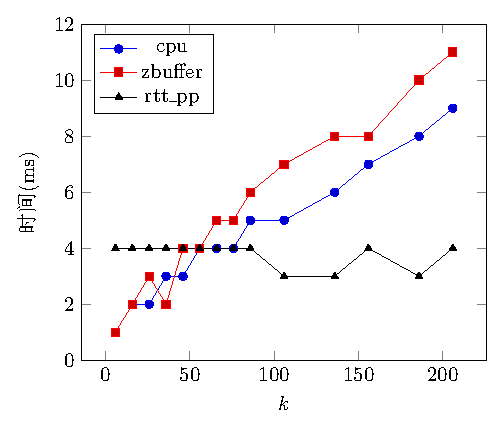
\includegraphics[width=\fourgraphicswidth\textwidth,page=1]{shadertime.pdf}
}
\subcaptionbox{Buddha模型(31232个点)\label{fig:exp:shader:buddha}}
{  
    \includegraphics[width=\fourgraphicswidth\textwidth, page=2]{shadertime.pdf}
}\linebreak %强制换行
\subcaptionbox{Alice模型(224291个点)\label{fig:exp:shader:alice}}
{  
   \includegraphics[width=\fourgraphicswidth\textwidth, page=3]{shadertime.pdf}
}
\subcaptionbox{Bugatti模型(1010815个点)\label{fig:exp:shader:buggatti}}
{  
   \includegraphics[width=\fourgraphicswidth\textwidth, page=4]{shadertime.pdf}
}
\caption{基于着色器的并行算法运行时间}
\label{fig:chart:exps:shadertime}
\end{figure}

从实验结果可以看出,当模型规模不大时,如图~\ref{fig:exp:shader:apple}~所示的含有8千多个点的~Apple~模型,
Z Buffer~算法和传统的~CPU~算法差别不是很大,因此在实际应用中当模型规模较小时可直接用~CPU~计算即可。
随着输入模型所含有点的数量规模的增加,CPU~和~GPU~运行时间之间的差距也越来越大。
当多面体面数增加即~$k$~的增大时,在~Z Buffer~算法中,需要更多的绘制次数,因此其运行时间也有所增加,而在基于乒乓技术的算法中,当点规模一定时,$k$~的变化对最后运行时间影响不明显,因此当较大的~$k$~时,这种算法更快。

\begin{table}[htbp]
\centering
\caption{基于着色器并行算法加速比}
\label{tab:exper:shadertime}
\begin{minipage}[t]{0.8\textwidth}
  \begin{tabular}{p{1.5cm}<{\centering}cccc cccc} %p本身占一列
  \toprule[1.5pt]
  \multirow{2}{*}{$k$} & \multicolumn{4}{c}{Apple模型(8118 个点)} &
  \multicolumn{4}{c}{Bugatti~模型(1010815个点)}\\
  \cmidrule(lr){2-5}\cmidrule(lr){6-9}
  ~&cpu & Z buffer  & rtt\_pp & 加速比$^{(a)}$ & cpu  & Z buffer& rtt\_pp& 加速比 \\
  \midrule[1pt]
 6	 & 6 	& 5 	& 41 &	1.20 &	26	& 17	&178  &	1.53 \\
16	 & 16	& 13	& 43 &	1.23 &	70	& 48	&181  &	1.46 \\
26	 & 25	& 17	& 43 &	1.47 &	114	& 68	&183  &	1.68 \\
36	 & 34	& 17	& 45 &	2.00 &	153	& 70	&178  &	2.19 \\
46	 & 44	& 24	& 42 &	1.83 &	203	& 102	&176  &	1.99 \\
56	 & 53	& 31	& 43 &	1.71 &	241	& 131	&177  &	1.84 \\
66	 & 62	& 39	& 43 &	1.59 &	285	& 162	&179  &	1.76 \\
76	 & 73	& 46	& 46 &	1.59 &	331	& 196	&189  &	1.75 \\
86	 & 82	& 52	& 45 &	1.82 &	373	& 225	&192  &	1.94 \\
106	 & 100	& 59	& 45 &	2.22 &	464	& 257	&191  &	2.43 \\
136	 & 127	& 81	& 42 &	3.02 &	604	& 349	&180  &	3.36 \\
156	 & 146	& 88	& 47 &	3.11 &	693	& 378	&202  &	3.43 \\
186	 & 177	& 110	& 43 &	4.12 &	861	& 474	&180  &	4.78 \\
206	 & 194	& 123	& 49 &	3.96 &	962	& 533	&209  &	4.60 \\
  \bottomrule[1.5pt]
\end{tabular}\\[2pt]
  \footnotesize (a): 加速比=~cpu/$min$(Z buffer, rtt\_pp)
\end{minipage}
\end{table}

表~\ref{tab:exper:shadertime}~详细的展示了基于着色器的两种算法应用于~Alice~和~Bugatti~模型的构造时间及相应的加速比。
从中可看出,Z Buffer~算法适合相对较小的~$k$~值,而基于乒乓技术的算法在较大~$k$~值时能达到更大的加速比。

本文实现了文献~\onlinecite{karlsson2010parallel}~中的并行算法并进行对比实验,表~\ref{tab:exp:sse-time}
~为实验统计结果,表中数据均为搜索截面耗时,因为二者其他步骤均相同且从~\ref{fig:chart:exps:cputime}~可得搜索截面时间占用整体绝大部分时间,其中~$k$~为多面体面数,
列~SSE~和列~$k$-CBP~分别为文献~\onlinecite{karlsson2010parallel}~中的算法和本文提出的基于~CUDA~算法的运行时间(单位毫秒)。

\begin{table}[htbp] 
\centering
\caption{本文算法与文献~\onlinecite{karlsson2010parallel}~的并行算法对比}
\begin{tabular}{p{1.5cm}<{\centering}ccc ccc} %p本身占一列
\toprule[1.5pt]
\multirow{2}{*}{$k$} & \multicolumn{3}{c}{Apple模型(8118个点)} &
\multicolumn{3}{c}{Bugatti~模型(1010815个点)}\\
\cmidrule(lr){2-4}\cmidrule(lr){5-7}
~&SSE\cite{karlsson2010parallel} & $k$-CBP &  加速比 & SSE\cite{karlsson2010parallel} & $k$-CBP &  加速比\\
\midrule[1pt]
6 & 0.4 & 0.12  & 3.20     & 24.2 & 3.20  & 7.56 \\
16 & 0.9 & 0.26  & 3.43    & 44.5 & 8.44  & 5.27 \\
26 & 1.4 & 0.41  & 3.38    & 66.5 & 13.65  & 4.87 \\
36 & 1.9 & 0.52  & 3.65    & 91.1 & 18.34  & 4.97 \\
46 & 2.5 & 0.67  & 3.74    & 119.5 & 24.13  & 4.95 \\
56 & 2.9 & 0.79  & 3.66    & 138.4 & 28.86  & 4.80 \\
66 & 3.5 & 0.95  & 3.69    & 170.6 & 34.10  & 5.00 \\
76 & 4.0 & 1.08  & 3.70    & 197.1 & 39.85  & 4.95 \\
86 & 4.5 & 1.22  & 3.69    & 219.8 & 45.08  & 4.88 \\
106 & 5.4 & 1.49  & 3.62   & 267.8 & 55.52  & 4.82 \\
136 &  6.8 & 1.92  & 3.54  & 342.9 & 71.24  & 4.81 \\
156 &  7.7 & 2.17  & 3.55  & 411.3 & 81.18  & 5.07 \\
186 &  9.3 & 2.60  & 3.58  & 479.4 & 97.39  & 4.92 \\
206 &  10.5 & 2.85  & 3.68 & 523.0 & 106.87  & 4.89  \\  
\bottomrule[1.5pt]
\end{tabular}
\label{tab:exp:sse-time}
\end{table}

与文献~\onlinecite{karlsson2010parallel}~中的算法相比,本文算法优势明显。
当用于点数量较小~Apple~模型时,能够提高~3$\sim$4~倍速度,模型变大,加速比也更大,~Bugatti~模型的提速达到~4$\sim$8~倍。

\subsection{凸包围多面体紧致程度}
\label{subsec:exper:tightness}

凸包围多面体的质量用公式(\ref{equa:judge:tightness})衡量即通过凸包与凸包围多面体的体积之比来量化包围体的紧致程度。
文献~\onlinecite{abenchmarking2007}~是基于~$k$-DOP~实现的层次结构的包围体,其顶层的~$k$-DOP~与本文算法生成的~$k$-CBP~的紧致程度对比如图~\ref{chart:exps:tightness}~所示,
图中横坐标~$k$~为凸包围多面体的面数,纵坐标为紧致程度,曲线~$k$-DOP~和~$k$-CBP~分别为文献~\onlinecite{abenchmarking2007}~和本文的方法,由图可知,
对于不同模型,本文构造的凸包围多面体紧致程度均有所提升,如~Alice~模型提升了12.08\%,~Dinasour~模型提升了34.0\%。
以~$k \in {20,38}$~为例,相应模型的~$k$-DOP~和~$k$-CBP~效果可见图~\ref{fig:kdop:kcbp:ui}。

\begin{figure}[htbp] 
\centering
\subcaptionbox{Apple(8118个点)\label{fig:exp:apple}}
{
    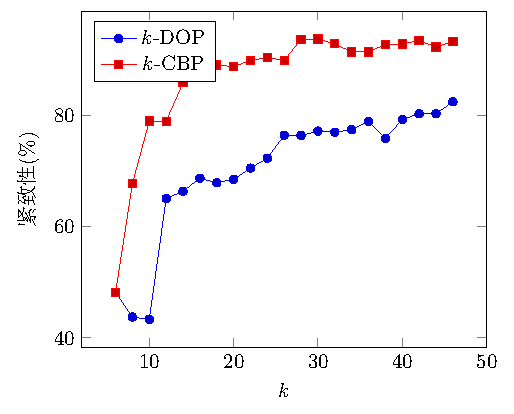
\includegraphics[width=\fourgraphicswidth\textwidth,page=1]{tightness.pdf}
}
\subcaptionbox{Budda(31232个点)\label{fig:exp:budda}}
{  
   \includegraphics[width=\fourgraphicswidth\textwidth,page=2]{tightness.pdf}
}
\linebreak
\subcaptionbox{Dinosaur(40277个点)\label{fig:exp:Dinasour}}
{  
    \includegraphics[width=\fourgraphicswidth\textwidth, page=3]{tightness.pdf}
}
\subcaptionbox{Alice(224291个点)\label{fig:exp:alice}}
{  
   \includegraphics[width=\fourgraphicswidth\textwidth, page=4]{tightness.pdf}
}
\caption{紧致程度对比:$k$-DOP~为文献~\onlinecite{abenchmarking2007}~的算法, $k$-CBP~为本文算法}
\label{chart:exps:tightness}
\end{figure}

\begin{figure}[htbp] 
\centering
\subcaptionbox{Bunny(20-DOP)\label{fig:exp:bunny:20dop}}
{  
   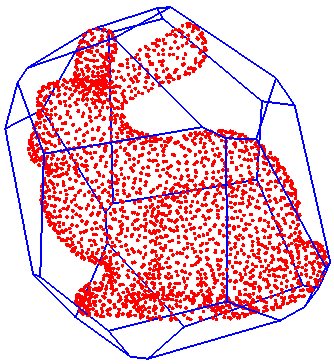
\includegraphics[width=0.21\textwidth]{bunny-kDOP-20.png}
}
\subcaptionbox{Bunny(20-CBP)\label{fig:exp:bunny:20cbp}}
{
    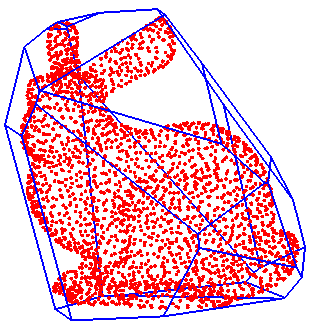
\includegraphics[width=0.21\textwidth]{bunny-kCBP-20.png}
}
\subcaptionbox{Bunny(38-DOP)\label{fig:exp:bunny:38dop}}
{  
   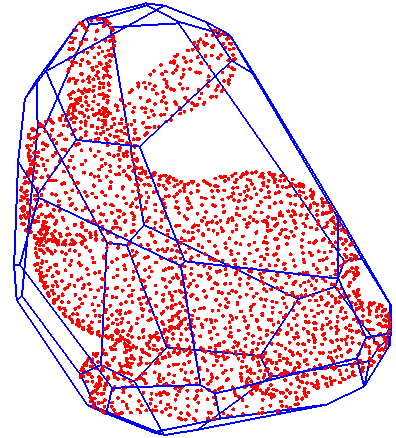
\includegraphics[width=0.21\textwidth]{bunny-kDOP-38.png}
}
\subcaptionbox{Bunny(38-CBP)\label{fig:exp:bunny:38cbp}}
{  
   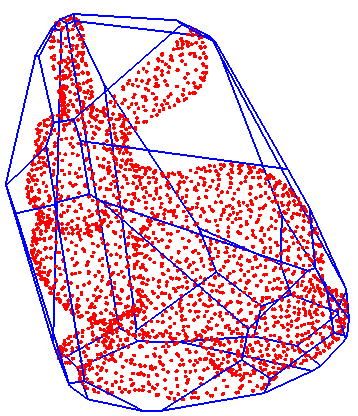
\includegraphics[width=0.21\textwidth]{bunny-kCBP-38.png}
}
\linebreak
\subcaptionbox{Apple(20-DOP)\label{fig:exp:apple:20dop}}
{  
   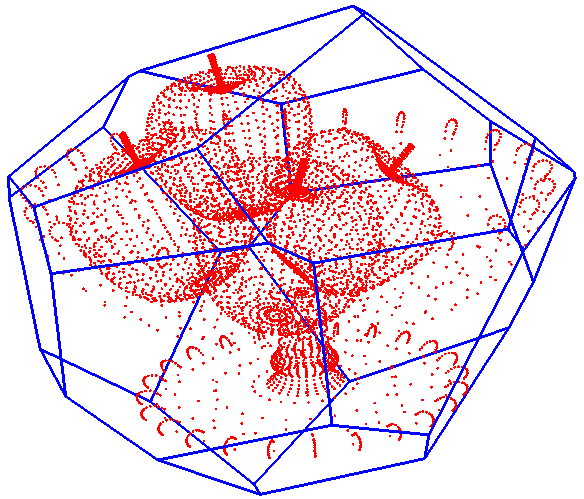
\includegraphics[width=0.21\textwidth]{apple3-kDOP-20.png}
}
\subcaptionbox{Apple(20-CBP)\label{fig:exp:apple:20cbp}}
{
    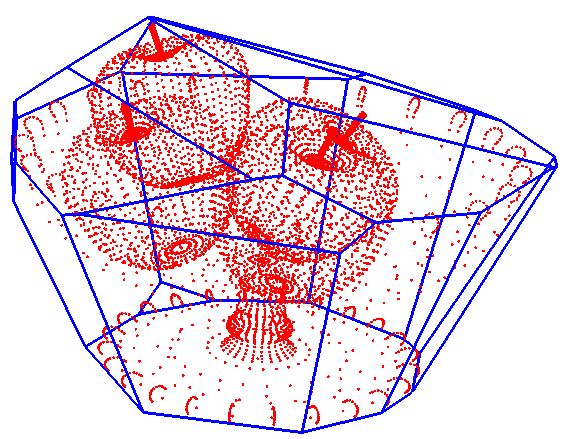
\includegraphics[width=0.21\textwidth]{apple3-kCBP-20.png}
}
\subcaptionbox{Apple(38-DOP)\label{fig:exp:apple:38dop}}
{  
   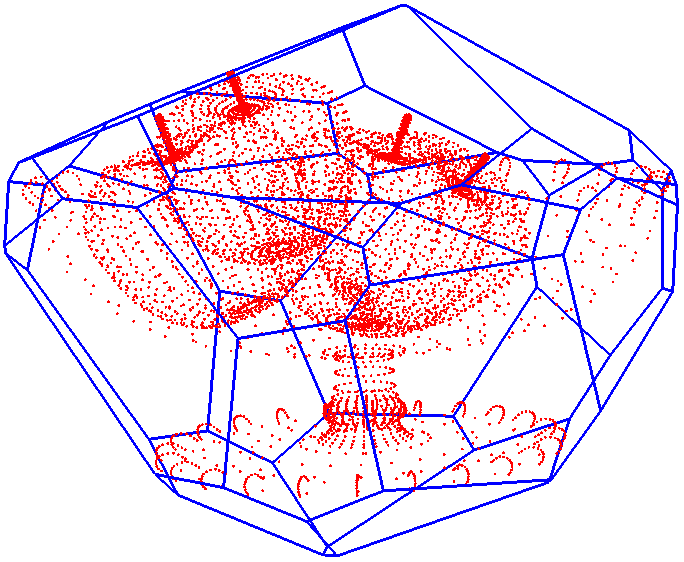
\includegraphics[width=0.21\textwidth]{apple3-kDOP-38.png}
}
\subcaptionbox{Apple(38-CBP)\label{fig:exp:apple:38cbp}}
{  
   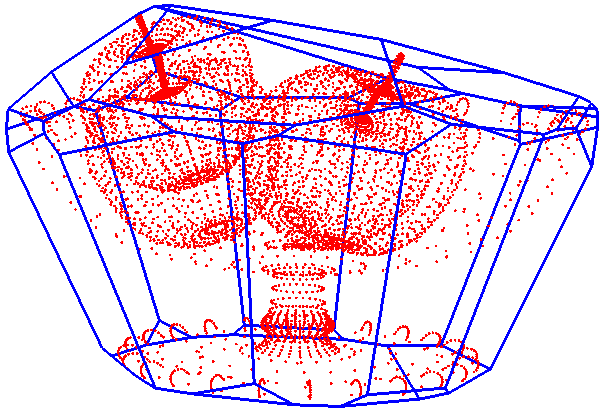
\includegraphics[width=0.21\textwidth]{apple3-kCBP-38.png}
}
\linebreak
\subcaptionbox{Budda(20-DOP)\label{fig:exp:Budda:20dop}}
{  
   \includegraphics[width=0.20\textwidth]{Budda-kDOP-20.png}
}
\subcaptionbox{Budda(20-CBP)\label{fig:exp:Budda:20cbp}}
{
    \includegraphics[width=0.20\textwidth]{Budda-kCBP-20.png}
}
\subcaptionbox{Budda(38-DOP)\label{fig:exp:Budda:38dop}}
{  
   \includegraphics[width=0.20\textwidth]{Budda-kDOP-38.png}
}
\subcaptionbox{Budda(38-CBP)\label{fig:exp:Budda:38cbp}}
{  
   \includegraphics[width=0.20\textwidth]{Budda-kCBP-38.png}
}
\linebreak
\subcaptionbox{Dinosaur(20-DOP)\label{fig:exp:Dinosaur:20dop}}
{  
  \includegraphics[height=2.8cm, width=0.23\textwidth]{Dinosaur-kDOP-20.png}
}
\subcaptionbox{Dinosaur(20-CBP)\label{fig:exp:Dinosaur:20cbp}}
{
  \rotatebox{0}{\includegraphics[height=2.8cm, width=0.23\textwidth]{Dinosaur-kCBP-20.png}}
}
\subcaptionbox{Dinosaur(38-DOP)\label{fig:exp:Dinosaur:38dop}}
{  
  \rotatebox{0}{\includegraphics[height=2.8cm, width=0.23\textwidth]{Dinosaur-kDOP-38.png}}
}
\subcaptionbox{Dinosaur(38-CBP)\label{fig:exp:Dinosaur:38cbp}}
{  
  \rotatebox{0}{\includegraphics[height=2.8cm, width=0.23\textwidth]{Dinosaur-kCBP-38.png}}
}
\linebreak
\subcaptionbox{Alice(20-DOP)\label{fig:exp:Alice:20dop}}
{  
   \includegraphics[width=0.20\textwidth]{Alice-kDOP-20.png}
}
\subcaptionbox{Alice(20-CBP)\label{fig:exp:Alice:20cbp}}
{
    \includegraphics[width=0.20\textwidth]{Alice-kCBP-20.png}
}
\hspace{1em}
\subcaptionbox{Alice(38-DOP)\label{fig:exp:Alice:38dop}}
{  
   \includegraphics[width=0.20\textwidth]{Alice-kDOP-38.png}
}
\subcaptionbox{Alice(38-CBP)\label{fig:exp:Alice:38cbp}}
{  
   \includegraphics[width=0.20\textwidth]{Alice-kCBP-38.png}
}
\caption{~$k$-CBP~与~$k$-DOP~对比}
\label{fig:kdop:kcbp:ui}
\end{figure}

本文算法利用近似凸包与精确凸包的相似性,从近似凸包的众多面片对应的法向中通过~$k$-means~聚类算法生成~$k$~个法向。
表~\ref{tab:exp:ach:ch:tightness}~为利用~Alice~模型的近似凸包和精确凸包分别聚类生成法向构造~$k$-CBP~的紧致程度对比。
可以看出,一方面,利用精确凸包构造的~$k$-CBP~并不一定比近似凸包构造的结果更紧致,但由于近似凸包与精确凸包的外观的近似性因此二者得到的结果相差并不大(5\%以内);
另一方面,因近似凸包的时间复杂度为线性,而精确凸包为~$O(n\log n)$,
因此本文利用近似凸包聚类生成法向。示例中构造近似凸包耗费时间仅为~0.88ms~,而精确凸包为~79.31ms~。

\begin{table}[!ht]   
\centering
\caption{用近似凸包与精确凸包构造~$k$-CBP~紧致程度对比}
\label{tab:exp:ach:ch:tightness}
\begin{tabular}{lccccl}
\toprule[1.5pt]
$k$ &  $\tau$(ACHull)(\%) & $\tau$ (CHull)(\%)  & $k$ &  $\tau$ (ACHull)(\%) & $\tau$ (CHull)(\%) \\
\midrule[1.0pt]
10 &	70.44 & 	65.56     &26 &	89.93 & 	94.45 \\
12 &	74.56 & 	75.63     &28 &	88.61 & 	92.24 \\
14 &	79.50 & 	82.49     &30 &	91.58 & 	92.35 \\
16 &	84.79 & 	85.20     &32 &	92.78 & 	93.78 \\
18 &	85.75 & 	90.09     &34 &	91.28 & 	93.22 \\
20 &	86.38 & 	90.36     &36 &	92.93 & 	94.68 \\
22 &	90.27 & 	92.48     &38 &	93.41 & 	93.20 \\
24 &	90.70 & 	93.09     &40 &	93.81 & 	94.70 \\
\bottomrule[1.5pt]
\end{tabular}
\end{table}

\begin{table}[htbp] 
\centering
\caption{$k$-CBP~与~QuickHull~凸包算法比较}
\label{tab:exp:cgal}
\begin{tabular}{lcccccl}
\toprule[1.5pt]
 Model & $f$(CHull)& $f$($k$-CBP) & $\tau$ ($k$-CBP)(\%) & $t$(CHull)(ms) & $t$($k$-CBP)(ms)\\ % 后面重新跑的, KCBP加上了近似凸包及求交时间的总和, 和近似凸包的分组时间也加了.
\midrule[1.0pt]
  Apple	& 499 & 30 & 93.67 & 5.5 & 1.30 \\ % apple3  自己电脑跑的数据, 之前是用的chengxianyu的电脑.
  Budda	& 1608 & 46 & 92.39 & 21.3 & 2.86 \\ %  1.0+0.86+1
  Dinosaur	& 1240 & 44 & 93.34 & 22.6 & 1.99 \\  % 1.0+0.98+0.1
  Alice	& 1332 & 44 & 93.92 & 85.8 & 8.47\\ % 2+6.48
  Bugatti & 24654 & 44 & 95.06 & 688.7 & 25.41 \\
\bottomrule[1.5pt]
\end{tabular}
\end{table}


%\begin{figure}[htbp] 
%\centering
%\subcaptionbox{Dinasour(44-CBP)\label{fig:exp:dinosaur}}
%{
%    \rotatebox{0}{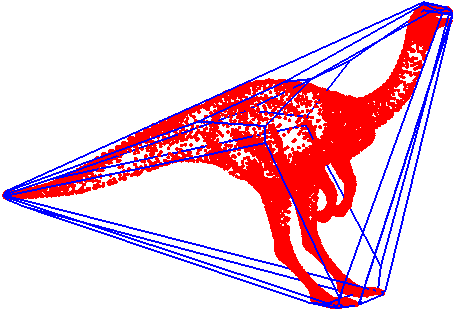
\includegraphics[width=0.38\textwidth]{dinosaur-44-w-n.png}}
%}
%\subcaptionbox{Dinosaur(CHull)\label{fig:exp:ch:dinosaur}}
%{  
%    \rotatebox{0}{\includegraphics[width=0.40\textwidth]{dinosaur-convexhull.png}}
%}
%\linebreak
%\subcaptionbox{Bugatti(44-CBP)\label{fig:exp:buggati}}
%{  
%   \includegraphics[width=0.40\textwidth]{buggati-44-w-n.png}
%}
%\subcaptionbox{Bugatti(CHull)\label{fig:exp:ch:buggati}}
%{  
%   \includegraphics[width=0.40\textwidth]{bugatti-convexhull.png}
%}
%\linebreak
%\subcaptionbox{Alice(44-CBP)\label{fig:exp:alice}}
%{  
%   \includegraphics[width=0.25\textwidth]{alice-44-w-n.png}
%}
%\subcaptionbox{Apple(30-KCBP)\label{fig:exp:apple}}
%{
%    \includegraphics[width=0.35\textwidth]{apple-30-w-n.png}
%}
%\subcaptionbox{Budda(46-CBP)\label{fig:exp:budda}}
%{  
%   \includegraphics[width=0.25\textwidth]{budda-46-w-n.png}
%}
%\linebreak
%\subcaptionbox{Alice(CHull)\label{fig:exp:ch:alice}}
%{  
%   \includegraphics[width=0.25\textwidth]{alice-convexhull.png}
%}
%\subcaptionbox{Apple(CHull)\label{fig:exp:ch:apple}}
%{
%    \includegraphics[width=0.34\textwidth]{apple-convexhull.png}
%}
%\subcaptionbox{Budda(CHull)\label{fig:exp:ch:budda}}
%{  
%   \includegraphics[width=0.25\textwidth]{budda-convexhull.png}
%}
%\caption{~$k$-CBP~与凸包对比}
%\label{pic:exps:ch-kcbp}
%\end{figure}

\begin{figure}[htbp] 
\centering
\subcaptionbox{Alice(44-CBP)\label{fig:exp:alice}}
{  
   \includegraphics[width=0.20\textwidth]{alice-44-w-n.png}
}
\subcaptionbox{Apple(30-KCBP)\label{fig:exp:apple}}
{
    \includegraphics[width=0.28\textwidth]{apple-30-w-n.png}
}
\subcaptionbox{Bugatti(44-CBP)\label{fig:exp:buggati}}
{  
  \rotatebox{-80}{\includegraphics[width=0.32\textwidth]{buggati-44-w-n.png}}
}
\subcaptionbox{Budda(46-CBP)\label{fig:exp:budda}}
{  
   \includegraphics[width=0.20\textwidth]{budda-46-w-n.png}
}
\linebreak
\subcaptionbox{Alice(CHull)\label{fig:exp:ch:alice}}
{  
   \includegraphics[width=0.20\textwidth]{alice-convexhull.png}
}
\subcaptionbox{Apple(CHull)\label{fig:exp:ch:apple}}
{
    \includegraphics[width=0.28\textwidth]{apple-convexhull.png}
}
\subcaptionbox{Bugatti(CHull)\label{fig:exp:ch:buggati}}
{  
  \rotatebox{-80}{\includegraphics[width=0.32\textwidth]{bugatti-convexhull.png}}
}
\subcaptionbox{Budda(CHull)\label{fig:exp:ch:budda}}
{  
   \includegraphics[width=0.20\textwidth]{budda-convexhull.png}
}
\linebreak
\subcaptionbox{Dinasour(44-CBP)\label{fig:exp:dinosaur}}
{
    \rotatebox{0}{\includegraphics[width=0.38\textwidth]{dinosaur-44-w-n.png}}
}
\subcaptionbox{Dinosaur(CHull)\label{fig:exp:ch:dinosaur}}
{  
    \rotatebox{0}{\includegraphics[width=0.40\textwidth]{dinosaur-convexhull.png}}
}
\caption{~$k$-CBP~与凸包对比}
\label{pic:exps:ch-kcbp}
\end{figure}

\clearpage
本文算法与~CGAL~库中利用~QuickHull~算法构造的凸包进行比较的结果如表~\ref{tab:exp:cgal}~所示,
其中~$f$(CHull)~和~$f$($k$-CBP)~分别表示凸包的面数和凸包围多面体的面数,$\tau$($k$-CBP)~为凸包围多面体的紧致程度,$t$(CHull)~和~$t$($k$-CBP)~分别表示凸包和~$k$-CBP~构造所花费的时间。
相应模型的可视化结果如图~\ref{pic:exps:ch-kcbp}~所示。
与凸包相比,本文算法在大大简化包围体平面数量的同时能保持较好的紧致程度,例如~Apple~模型的凸包有~499~个平面,本文算法仅用~30~个平面就能达到~93.67\%的紧致程度,
而对~Bugatti~模型,仅用了其凸包平面数量的0.17\%就达到95.06\%的紧致程度,且构造速度快了~27~倍。

\FloatBarrier
\section{本章小结}
\label{sec:chap02:summary}

本章主要介绍了凸包围多面体~$k$-CBP~的生成算法,算法主要分为3个步骤,
首先确定生成的~$k$-CBP~的法向,为了得到更加紧致的凸包围多面体,本文利用~$k$-means~对构造的近似内凸包的法向进行聚类;
然后多次扫描模型点集得到每个法向的切点进而得到截面,该过程各方向计算相互独立互不影响,因此利用了~GPU~进行加速;
最后通过截面求交得到~$k$-CBP~的各个顶点。
本章最后通过实验从凸包围多面体的生成效率和紧致程度两个角度与现有算法进行对比,说明本文算法能够快速构造更加紧致的凸包围多面体,效率上平均能够提高~3 $\sim$ 8~倍,且较~$k$-DOP~提高了近~10\% $\sim$ 40\%~的紧致程度。

